\documentclass[tikz]{standalone}
\usetikzlibrary {positioning,shapes.misc}\begin{document}
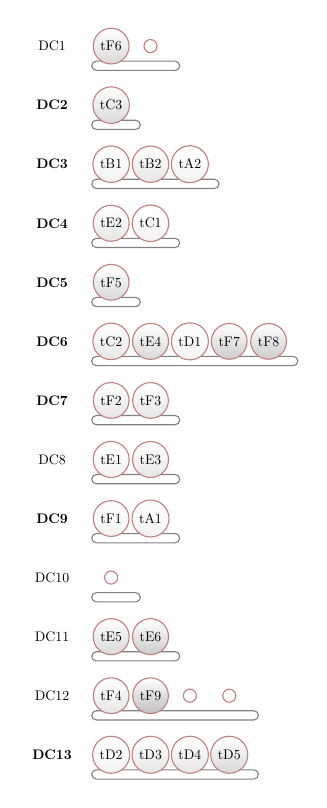
\begin{tikzpicture}[scale=0.5, every node/.style={scale=0.5}]

\tikzstyle{dc} = [rounded rectangle,right,draw=gray,yshift=-0.5cm];
\tikzstyle{task} = [circle,draw=red!50!black!50,top color=white];
\tikzstyle{dp}=[draw,opacity=0.3]
\node at (-1.5,0) {DC1};
\node[dc,text width=2.0cm] (DC1) at (-0.5,0) {};
\node[task,bottom color=black!15.0] at (0,0) {tF6};
\node[task] at (1,0) {};
\node[font=\bfseries] at (-1.5,-1.5) {DC2};
\node[dc,text width=1.0cm] (DC2) at (-0.5,-1.5) {};
\node[task,bottom color=black!15.0] at (0,-1.5) {tC3};
\node[font=\bfseries] at (-1.5,-3.0) {DC3};
\node[dc,text width=3.0cm] (DC3) at (-0.5,-3.0) {};
\node[task,bottom color=black!5.0] at (0,-3.0) {tB1};
\node[task,bottom color=black!10.0] at (1,-3.0) {tB2};
\node[task,bottom color=black!5.0] at (2,-3.0) {tA2};
\node[font=\bfseries] at (-1.5,-4.5) {DC4};
\node[dc,text width=2.0cm] (DC4) at (-0.5,-4.5) {};
\node[task,bottom color=black!10.0] at (0,-4.5) {tE2};
\node[task,bottom color=black!5.0] at (1,-4.5) {tC1};
\node[font=\bfseries] at (-1.5,-6.0) {DC5};
\node[dc,text width=1.0cm] (DC5) at (-0.5,-6.0) {};
\node[task,bottom color=black!15.0] at (0,-6.0) {tF5};
\node[font=\bfseries] at (-1.5,-7.5) {DC6};
\node[dc,text width=5.0cm] (DC6) at (-0.5,-7.5) {};
\node[task,bottom color=black!10.0] at (0,-7.5) {tC2};
\node[task,bottom color=black!15.0] at (1,-7.5) {tE4};
\node[task,bottom color=black!5.0] at (2,-7.5) {tD1};
\node[task,bottom color=black!20.0] at (3,-7.5) {tF7};
\node[task,bottom color=black!20.0] at (4,-7.5) {tF8};
\node[font=\bfseries] at (-1.5,-9.0) {DC7};
\node[dc,text width=2.0cm] (DC7) at (-0.5,-9.0) {};
\node[task,bottom color=black!10.0] at (0,-9.0) {tF2};
\node[task,bottom color=black!10.0] at (1,-9.0) {tF3};
\node at (-1.5,-10.5) {DC8};
\node[dc,text width=2.0cm] (DC8) at (-0.5,-10.5) {};
\node[task,bottom color=black!5.0] at (0,-10.5) {tE1};
\node[task,bottom color=black!10.0] at (1,-10.5) {tE3};
\node[font=\bfseries] at (-1.5,-12.0) {DC9};
\node[dc,text width=2.0cm] (DC9) at (-0.5,-12.0) {};
\node[task,bottom color=black!5.0] at (0,-12.0) {tF1};
\node[task,bottom color=black!5.0] at (1,-12.0) {tA1};
\node at (-1.5,-13.5) {DC10};
\node[dc,text width=1.0cm] (DC10) at (-0.5,-13.5) {};
\node[task] at (0,-13.5) {};
\node at (-1.5,-15.0) {DC11};
\node[dc,text width=2.0cm] (DC11) at (-0.5,-15.0) {};
\node[task,bottom color=black!15.0] at (0,-15.0) {tE5};
\node[task,bottom color=black!20.0] at (1,-15.0) {tE6};
\node at (-1.5,-16.5) {DC12};
\node[dc,text width=4.0cm] (DC12) at (-0.5,-16.5) {};
\node[task,bottom color=black!10.0] at (0,-16.5) {tF4};
\node[task,bottom color=black!25.0] at (1,-16.5) {tF9};
\node[task] at (2,-16.5) {};
\node[task] at (3,-16.5) {};
\node[font=\bfseries] at (-1.5,-18.0) {DC13};
\node[dc,text width=4.0cm] (DC13) at (-0.5,-18.0) {};
\node[task,bottom color=black!5.0] at (0,-18.0) {tD2};
\node[task,bottom color=black!10.0] at (1,-18.0) {tD3};
\node[task,bottom color=black!10.0] at (2,-18.0) {tD4};
\node[task,bottom color=black!15.0] at (3,-18.0) {tD5};
\end{tikzpicture}
\end{document}
